% Provenance (never printed): see sources/outline_sources.md (Year 2: Hadean, Archean and
% Proterozoic; early crust and greenstone belts; the oxygenation of the atmosphere; snowball
% Earth). Eons and eras from the ICS chart; greenstone belts, TTG and cratons after Cawood and
% others (2018) and Smithies and others (2019); komatiite liquidus after Sossi and O'Neill (2016),
% Pierru and others (2022) and Asimow (2022); the Archean air and the GOE after Catling and Zahnle
% (2020) and Luo and others (2016); the boring billion after Lyons and others (2021); snowball
% Earth after Hoffman and others (2017). The energy-balance model, the komatiite line and the CO2
% build-up from figdata/bachelor-2/precambrian.py; exercise and problem values in the Book 4
% scratch calculator calc/ch18.py.
\chapter{الأرض فيما قبل الكمبري}\label{ch:b2:precambrian-earth}

تظهر أولى الأحافير ذات الأصداف في صخور عمرها نحو 540 مليون سنة. وكلّ ما قبلها، منذ
ولادة الأرض قبل \qty{4567}{Ma}، هو ما قبل الكمبري: سبعة أثمان تاريخ
الكوكب. وفي ذلك الزمن بنت الأرض نوى قارّاتها، وملأت هواءها بالأكسجين،
وتجمّدت مرّتين على الأقلّ من القطبين إلى خطّ الاستواء، وبلغت صفائحها الجليدية البحر
في المناطق المدارية. يقرأ هذا الفصل تلك المليارات الأربعة من السنين في الصخور الباقية منها،
ويضع أرقامًا على ثلاثة من ألغازها: لماذا كانت أقدم الحمم بهذه الحرارة، وكيف يمكن لكوكب
متجمّد أن يذوب، وكيف بقيت الأرض الفتيّة دافئة تحت شمس خافتة.
% ledger: ics:base.Hadean, ics:base.Phanerozoic, hoffman17:cryochrons

\begin{recall}
\textbf{من مجلدات المدرسة}: عمر الأرض؛ والدهور في السلّم الزمني الجيولوجي؛
وقانون سطوع الشمس الفتيّة \omterm{def:b2:precambrian-earth:faint-sun}{ومشكلة الشمس الفتية الخافتة}؛ والغلاف الجوي البدائي؛
والستروماتوليتات، وتكوينات الحديد الشريطية، \omterm{def:b2:precambrian-earth:goe}{وحدث الأكسدة العظيم} والطبقات الحمراء؛ والكراتونات؛
والحرارة الإشعاعية في الماضي. \textbf{من مجلد السنة الأولى}: الزركون وأعماره بطريقة اليورانيوم--الرصاص،
ودرجة الإغلاق؛ وإنتاج الحرارة الإشعاعي للنظائر الأربعة؛ والإشعاع طويل الموجة الخارج
والإشماس العالمي المتوسط $S_0/4$؛ والوحدات الكرونوستراتغرافية.
\textbf{من الفصول السابقة}: \omterm{def:b2:mantle-melting:tp}{درجة الحرارة الكامنة للوشاح} والتدرّج الكظوم
(\cref{ch:b2:mantle-melting})؛ وخطّ السيولة \omterm{def:b2:magmatic-differentiation:crystallisation}{والتبلور التجزيئي} للأوليفين
(\cref{ch:b2:magmatic-differentiation})؛ وأنواع الغرانيت (\cref{ch:b2:crustal-melting})؛
والقارّات العظمى (\cref{ch:b2:wilson-cycle}). أمّا الأكسدة والاختزال فتنتميان إلى مجلدات
الكيمياء، وأولى حقيقيات النوى والتركيب الضوئي إلى مجلدات الأحياء.
\end{recall}

\section{ثلاثة دهور قبل الأحافير}\label{sec:b2:precambrian-earth:eons}

\begin{definition}[الدهر الجهنمي، والدهر السحيق، ودهر الحياة الطليعية]\label{def:b2:precambrian-earth:eons}
ينقسم الزمن السابق لدهر الحياة الظاهرة إلى ثلاثة دهور. فيمتدّ \emph{الدهر الجهنمي}\index{الدهر الجهنمي}
من تكوّن الأرض، قبل \qty{4567}{Ma}، إلى $4031 \pm \qty{3}{Ma}$؛ ويمتدّ
\emph{الدهر السحيق}\index{الدهر السحيق} من $4031$ إلى \qty{2500}{Ma}؛ ويمتدّ
\emph{دهر الحياة الطليعية}\index{دهر الحياة الطليعية} من 2500 إلى \qty{538.8}{Ma}، أي قاعدة الكمبري.
وتُسمّى معًا، على نحو غير رسمي، ما قبل الكمبري.
\end{definition}
% ledger: ics:base.Hadean, ics:base.Archean, ics:base.Proterozoic, ics:base.Phanerozoic

وينقسم \omterm{def:b2:precambrian-earth:eons}{الدهر السحيق} إلى أربع حقب: السحيق الفجري (من 4031 إلى \qty{3600}{Ma})، والسحيق القديم (من 3600
إلى 3200)، والسحيق الأوسط (من 3200 إلى 2800) والسحيق الحديث (من 2800 إلى 2500)؛ وينقسم \omterm{def:b2:precambrian-earth:eons}{دهر الحياة الطليعية} إلى ثلاث:
الطليعي القديم (من 2500 إلى \qty{1600}{Ma})، والطليعي الأوسط (من 1600 إلى 1000)
والطليعي الحديث (من 1000 إلى 538.8). ويهمّنا أدناه عصران من الطليعي الحديث، الكريوجيني، من 720 إلى
\qty{635}{Ma}، والإدياكاري، من 635 إلى \qty{538.8}{Ma}.
% ledger: ics4:archean-eras, ics4:proterozoic-eras

\begin{omfigure}
\centering
% ledger: ics:base.Hadean, ics:base.Archean, ics:base.Proterozoic, ics:base.Phanerozoic, ics4:archean-eras, ics4:proterozoic-eras, wilde01:4404, bowring99:acasta, cz20:impacts, allwood06:spc, cawood18:transition, gumsley17:goe, luo16:goe, hoffman17:earlier, earle:bif, lyons21:boring, hoffman17:ages, asimow22:komatiite
\begin{tikzpicture}[x=-3.4cm, y=1cm, font=\scriptsize]
% eons
\fill[icsHadean] (4.567,0) rectangle (4.031,0.5);
\fill[icsArchean] (4.031,0) rectangle (2.5,0.5);
\fill[icsProterozoic] (2.5,0) rectangle (0.5388,0.5);
\fill[icsPhanerozoic] (0.5388,0) rectangle (0,0.5);
\node[text=white] at (4.299,0.25) {الدهر الجهنمي};
\node[text=white] at (3.27,0.25) {الدهر السحيق};
\node[text=white] at (1.52,0.25) {دهر الحياة الطليعية};
\node at (0.27,0.25) {\tiny الحياة الظاهرة};
% eras
\foreach \a/\b/\c in {4.031/3.6/35, 3.6/3.2/55, 3.2/2.8/35, 2.8/2.5/55}
  \fill[icsArchean!\c] (\a,-0.45) rectangle (\b,0);
\foreach \a/\b/\c in {2.5/1.6/35, 1.6/1.0/55, 1.0/0.5388/35}
  \fill[icsProterozoic!\c] (\a,-0.45) rectangle (\b,0);
\foreach \x/\l in {3.8155/فجري, 3.4/قديم, 3.0/أوسط, 2.65/حديث, 2.05/قديم, 1.3/أوسط, 0.769/حديث}
  \node at (\x,-0.225) {\l};
% axis
\draw (4.6,-0.6) -- (0,-0.6);
\foreach \t in {0,0.5,...,4.5} {
  \draw (\t,-0.6) -- (\t,-0.7);
  \node[anchor=north] at (\t,-0.7) {\pgfmathprintnumber[fixed, precision=1]{\t}};
}
\node[anchor=north, font=\small] at (2.3,-1.05) {الزمن قبل الحاضر (مليار سنة)};
% row A
\fill[omDef] (4.404,0.85) circle (2pt);
\node[anchor=west, text=omDef] at (4.404,0.85) {أقدم زركون};
\fill[omMeth] (3.43,0.85) circle (2pt);
\node[anchor=west, text=omMeth] at (3.43,0.85) {أولى الستروماتوليتات};
\draw[red!60!black, line width=3pt] (2.4,0.85) -- (1.8,0.85);
\node[anchor=west, text=red!60!black] at (1.8,0.85) {تكوينات الحديد الشريطية};
% row B
\fill[omDef] (4.03,1.5) circle (2pt);
\node[anchor=west, text=omDef] at (4.03,1.5) {أقدم الصخور};
\draw[black!70, line width=3pt] (3.2,1.5) -- (2.5,1.5);
\node[anchor=south, text=black!80] at (2.85,1.6) {تغيّر النمط التكتوني};
\draw[omProp, line width=3pt] (1.8,1.5) -- (0.8,1.5);
\node[anchor=south, text=omProp] at (1.3,1.6) {\foreignlanguage{arabic}{«المليار المملّ»}};
% row C
\draw[black!60, line width=2pt, densely dashed] (4.2,2.25) -- (3.5,2.25);
\node[anchor=south, text=black!70] at (3.85,2.35) {\foreignlanguage{arabic}{القصف الشديد المتأخّر؟ (موضع جدل)}};
\draw[omThm, line width=3pt] (2.43,2.25) -- (2.06,2.25);
\node[anchor=west, text=omThm] at (2.06,2.25) {حدث الأكسدة العظيم};
% row D
\fill[blue!60!black] (2.4,3.0) circle (2pt);
\node[anchor=east, text=blue!60!black] at (2.4,3.0) {أوّل أرض كرة ثلجية};
\fill[omThm] (0.8,3.0) circle (2pt);
\node[anchor=east, text=omThm] at (0.8,3.0) {الارتفاع الثاني للأكسجين};
% row E
\fill[orange!80!black] (1.9,3.7) circle (2pt);
\node[anchor=east, text=orange!80!black] at (1.9,3.7) {آخر الكوماتيتات الشائعة};
\draw[blue!60!black, line width=3pt] (0.717,3.7) -- (0.635,3.7);
\node[anchor=east, text=blue!60!black] at (0.717,3.7) {الأرض الكرة الثلجية في الكريوجيني};
% row F
\fill[omMeth] (0.57,4.4) circle (2pt);
\node[anchor=east, text=omMeth] at (0.57,4.4) {\foreignlanguage{arabic}{أولى الأحافير الكبيرة (الإدياكاري)}};
\end{tikzpicture}
\par\smallskip{\small ما قبل الكمبري على خطّ واحد. الدهور، وبألوان أفتح حقبها
(السحيق الفجري والقديم والأوسط والحديث؛ والطليعي القديم والأوسط والحديث)، هي دهور
الجدول الكرونوستراتغرافي الدولي وحقبه؛ والأحداث موضوعة عند الأعمار المذكورة في النص.
و«آخر الكوماتيتات الشائعة» هي غير المستنزَفة في الألومنيوم؛ وتوجد أنواع أحدث منها وأندر.}
\end{omfigure}

\subsection*{الدهر الجهنمي: معادن بلا صخور}

لا يبقى صخر من \omterm{def:b2:precambrian-earth:eons}{الدهر الجهنمي}، بل معادن فقط. وأقدمها حبّة زركون من تلال جاك
في غرب أستراليا، عمرها $4404 \pm \qty{8}{Myr}$، جُرفت من صخر أقدم ورسبت
في كونغلوميرات قبل نحو ثلاثة مليارات سنة. وقد قرأ مكتشفوها تركيبها، وتركيب
جاراتها، دليلًا على أن قشرة من النمط القاري وماءً سائلًا كانا موجودين منذ \qty{4.4}{Gyr}،
أي بعد نحو 160 مليون سنة من تكوّن الأرض. وأقدم الصخور المؤرَّخة، نيسات أكاستا في شمال غرب كندا،
يتراوح عمرها من 4.00 إلى \qty{4.03}{Ga}، قرب قاعدة \omterm{def:b2:precambrian-earth:eons}{الدهر السحيق}.
% ledger: wilde01:4404, wilde01:zircon, uw14:jack-hills, bowring99:acasta

تعرّضت الأرض الفتيّة لضربات أجسام كبيرة، كما وصف \cref{ch:b2:planet-formation-meteorites}.
ويُقدَّر أن آخر اصطدام كبير بما يكفي لتبخير المحيط كلّه وقع قبل نحو \qty{4.3}{Ga}.
وقد اقتُرح «قصف شديد متأخّر» لاحق، أي دفعة من الاصطدامات بين نحو 4.2--4.0 و\qty{3.5}{Ga} استُنتجت من
أعمار صخور القمر والصدمات في النيازك؛ ويشكّك كثيرون في أنه كان حدثًا
متميّزًا أصلًا، وعلى أيّ حال فالأرجح أنه لم يكن ليعقّم الأرض.
% ledger: cz20:impacts

\section{قشرة الدهر السحيق}\label{sec:b2:precambrian-earth:archean}

\subsection*{أحزمة الحجر الأخضر والكوماتيتات}

تتكوّن قشرة \omterm{def:b2:precambrian-earth:eons}{الدهر السحيق} الباقية من نوعين من الأراضي، جنبًا إلى جنب: أجسام كبيرة من
نيس غرانيتي رمادي غنيّ بالصوديوم، وأحزمة أضيق من صخور بركانية ورسوبية متحوّلة.

\begin{definition}[حزام الحجر الأخضر؛ الكوماتيت]\label{def:b2:precambrian-earth:greenstone}
\emph{حزام الحجر الأخضر}\index{حزام الحجر الأخضر} حزام من الصخور البركانية المافية وفوق المافية،
مع رواسب، متحوّل بدرجة منخفضة (يأتي اللون الأخضر من الكلوريت والأكتينوليت
والإبيدوت)، يقع بين أجسام من الغرانيتويد في أراضي \omterm{def:b2:precambrian-earth:eons}{الدهر السحيق} وبعض أراضي \omterm{def:b2:precambrian-earth:eons}{دهر الحياة الطليعية}.
و\emph{الكوماتيت}\index{الكوماتيت} حمم فوق مافية، أغنى بكثير بأكسيد المغنيسيوم من البازلت،
ثارت سائلةً؛ وينمو أوليفينها عادةً في شفرات طويلة رفيعة، هي نسيج
\emph{السبينيفكس}، إذ يبرد أعلى المسيل بسرعة.
\end{definition}
% ledger: cawood18:dome-keel, so16:liquidus, pierru22:komatiite

\begin{omfigure}
\centering
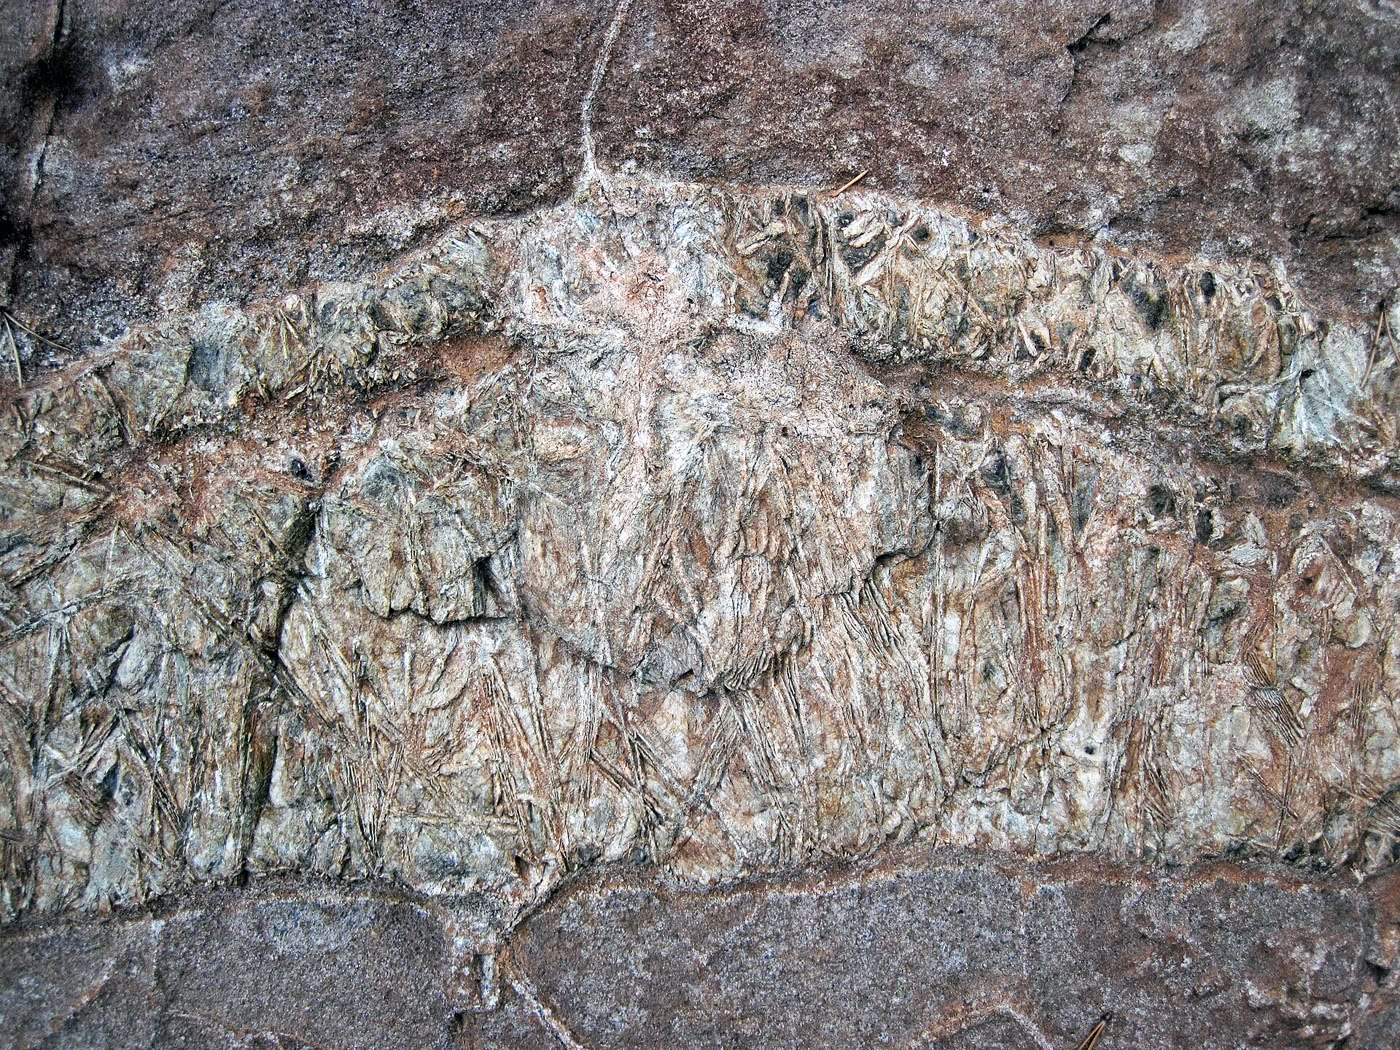
\includegraphics[width=0.66\linewidth]{images/book4/b2-18-spinifex-komatiite.jpg}
\par\smallskip{\small نسيج السبينيفكس في مسيل كوماتيتي، بايك هيل، أونتاريو، جزء من
حزام حجر أخضر من السحيق الحديث عمره نحو 2.71 مليار سنة: شفرات من الأوليفين، متبدّلة الآن،
نمت عبر الجزء الأعلى المتبرّد من المسيل. الصورة:
\mbox{\textdir TLT James St.~John, CC~BY~2.0 (Wikimedia Commons)}.}
\end{omfigure}

تحوي الكوماتيتات حتى \qty{34}{\percent} من أكسيد المغنيسيوم، مقابل 10 إلى \qty{13}{\percent} في البازلتات
الأوّلية لظهرات اليوم، وتكاد تقتصر على الأرض القديمة: فالنوع المستنزَف في الألومنيوم
لا يوجد إلا في صخور أقدم من \qty{2.8}{Ga}، والنوع غير المستنزَف في الألومنيوم حتى نحو
\qty{1.9}{Ga}، ولا يبلغ حداثة \qty{90}{Myr} إلا نوع نادر مُثرى بالألومنيوم. والمصهور
الغنيّ بالمغنيسيوم إلى هذا الحدّ حارّ جدًا، وكما في بازلتات
\cref{ch:b2:magmatic-differentiation}، فأوّل معدن يتبلور منه هو الأوليفين،
الذي تحدّد حصّته في السائل درجة الحرارة.
% ledger: pierru22:komatiite, asimow22:komatiite

\begin{proposition}[مقياس الحرارة الكوماتيتي]\label{prop:b2:precambrian-earth:liquidus}
من أجل مصهور في توازن مع الأوليفين عند الضغط الجوي، ترتفع درجة حرارة خطّ السيولة
ارتفاعًا شبه خطّي مع محتوى المصهور من أكسيد المغنيسيوم. وعبر تجربتين $(m_1, T_1)$
و$(m_2, T_2)$،
\[
  T_{\text{سائل}}(m) = T_1 + s\,(m - m_1), \qquad s = \frac{T_1 - T_2}{m_1 - m_2} .
\]
أعطت تجارب صهر على كوماتيتين، $\qty{32.2}{\percent}$ من أكسيد المغنيسيوم عند \qty{1616}{\celsius}
و$\qty{23}{\percent}$ عند \qty{1450}{\celsius}، القيمة $s = \qty{18.0}{\celsius}$ لكل واحد في المئة من
أكسيد المغنيسيوم.
\end{proposition}
% ledger: so16:liquidus, helz98:glass-thermometer

\begin{proof}
الأوليفين محلول صلب من الفورستيريت والفاياليت، أغنى بالمغنيسيوم بكثير من المصهور
الذي ينمو منه. ومع تبرّد المصهور يأخذ الأوليفين المغنيسيوم منه، فتنخفض درجة الحرارة التي
يكون عندها المصهور مشبعًا بالأوليفين بالكاد مع محتواه من أكسيد المغنيسيوم. وتُظهر التجارب أن
الانخفاض قريب من الخطّي على مدى عائلة معيّنة من المصاهير، فيستكمل الخطّ المارّ
بتجربتين ما بينهما؛ $s = (1616 - 1450)/(32.2 - 23) = 166/9.2 = 18.04$.
\end{proof}

ليس المعامل خاصًّا بالكوماتيتات. فالزجاج المسقى سريعًا من حمم كيلاويا،
المعايَر بالطريقة نفسها، يتغيّر بمقدار \qty{3}{\celsius} لكل \qty{0.15}{\percent} من أكسيد المغنيسيوم، أي
\qty{20}{\celsius} لكل واحد في المئة. ومدّ الخطّ الكوماتيتي حتى بازلت ظهرة أوّلي
فيه \qty{12}{\percent} من أكسيد المغنيسيوم يعطي إذن خطّ سيولته في حدود بضع عشرات من الدرجات: $1616 -
18.0\times20.2 \approx \qty{1252}{\celsius}$. فكانت أشدّ السوائل الكوماتيتية حرارةً
أسخن بنحو \qty{360}{\celsius} من المصاهير التي تغذّي ظهرات اليوم، ويبيّن الشكل أدناه
الخطّ.
% ledger: helz98:glass-thermometer, so16:liquidus, pierru22:komatiite
% values: slope 18.043, T_morb12 1251.5, dT_kom_morb 364.5 (precambrian.py)

\begin{omfigure}
\centering
\begin{tikzpicture}
\begin{axis}[omrecord, width=0.72\linewidth, height=6cm, xmin=8, xmax=35, ymin=1150, ymax=1700,
  xlabel={أكسيد المغنيسيوم في المصهور (\unit{\percent} كتليًا)}, ylabel={خطّ السيولة عند \babelsublr{1 atm} \babelsublr{(\unit{\celsius})}},
  xtick pos=bottom, ytick pos=left, clip=false,
  y tick label style={/pgf/number format/1000 sep={}}]
% computed in figdata/bachelor-2/precambrian.py part kom; ledger: so16:liquidus, pierru22:komatiite
\fill[omProp!15] (axis cs:10,1150) rectangle (axis cs:13,1700);
\addplot[black, line width=1.1pt] table[x=MgO, y=T] {figdata/out/bachelor-2-precambrian-kom.dat};
\addplot[only marks, mark=*, mark size=2.4pt, omThm] coordinates {(32.2,1616) (23,1450)};
\node[anchor=north west, font=\scriptsize, text=omThm] at (axis cs:32.2,1612) {باربرتون};
\node[anchor=north west, font=\scriptsize, text=omThm] at (axis cs:23,1446) {مونرو};
\node[anchor=south, font=\scriptsize, text=omProp, align=center] at (axis cs:11.5,1560)
  {بازلتات الظهرات\\الأوّلية};
\draw[densely dashed] (axis cs:12,1150) -- (axis cs:12,1251.5) -- (axis cs:8,1251.5);
\draw[densely dashed] (axis cs:32.2,1150) -- (axis cs:32.2,1616);
\draw[<->, omDef, thick] (axis cs:27,1251.5) -- (axis cs:27,1616);
\draw[densely dotted] (axis cs:12,1251.5) -- (axis cs:27,1251.5);
\draw[densely dotted] (axis cs:27,1616) -- (axis cs:32.2,1616);
\node[anchor=east, font=\scriptsize, text=omDef] at (axis cs:26.7,1330) {\foreignlanguage{arabic}{نحو \mbox{\textdir TLT \qty{360}{\celsius}}}};
\end{axis}
\end{tikzpicture}
\par\smallskip{\small مقياس الحرارة الكوماتيتي: الخطّ المارّ بدرجتي حرارة خطّ السيولة
المقيستين على كوماتيتين (النقطتان)، ممدودًا حتى 10 إلى \qty{13}{\percent} من أكسيد المغنيسيوم في البازلتات
الأوّلية لظهرات اليوم (النطاق). ويستند هذا المدّ إلى تشابه ميل المصاهير البازلتية.}
\end{omfigure}

الحمم الأسخن لا تعني وشاحًا أسخن بالمقدار نفسه. فالأرجح أن الكوماتيتات صعدت في
أعمدة، كما تفعل أسخن بازلتات اليوم في هاواي، حيث تعلو درجة الحرارة الكامنة حتى
نحو \qty{200}{\celsius} فوق $1350 \pm \qty{50}{\celsius}$ للوشاح المحيط. كما
تكوّنت بدرجات انصهار كبيرة، على عمق أكبر. ويُعتقد عمومًا أنها
تكوّنت في وشاح أدفأ من وشاح اليوم بمقدار 200 إلى \qty{300}{K}؛ ويرى رأي بديل أن
الكوماتيتات كانت صهارات مائية، تكوّنت عند درجات حرارة لا تزيد كثيرًا على الوشاح
المحيط. وعلى أيّ حال، كان وشاح \omterm{def:b2:precambrian-earth:eons}{الدهر السحيق} أسخن، وقد أعطت مجلدات
المدرسة سببًا لذلك: فقبل 3 مليارات سنة كانت النظائر المشعّة الأربعة تطلق أكثر من
ضعفي حرارة اليوم (\cref{exo:b2:precambrian-earth:2}).
% ledger: asimow22:komatiite, pierru22:komatiite, so16:liquidus

\subsection*{متتالية TTG ونمط القباب والعوارض}

النيسات الرمادية بين أحزمة الحجر الأخضر ليست غرانيتات من النوع الذي
وصفه \cref{ch:b2:crustal-melting}.

\begin{definition}[متتالية التوناليت--الترونجيميت--الغرانوديوريت]\label{def:b2:precambrian-earth:ttg}
\emph{متتالية التوناليت--الترونجيميت--الغرانوديوريت}\index{متتالية التوناليت--الترونجيميت--الغرانوديوريت} (TTG) هي عائلة الغرانيتويدات الغنيّة بالصوديوم والفقيرة بالبوتاسيوم --- التوناليتات،
والترونجيميتات (توناليتات فقيرة بالمعادن المافية) والغرانوديوريتات --- التي تكوّن معظم
القشرة القارية في \omterm{def:b2:precambrian-earth:eons}{الدهر السحيق}. وقد تكوّن معظمها \omterm{def:b2:mantle-melting:melting}{بالانصهار الجزئي} لقشرة بازلتية
مُميَّهة.
\end{definition}
% ledger: smithies19:ttg, cawood18:ttg

كان قسم كبير من حجم القشرة القارية الحالية قد تكوّن بنهاية \omterm{def:b2:precambrian-earth:eons}{الدهر السحيق}، ومعظمه
على هيئة TTG. وتحمل بعض صخور TTG بصمات من العناصر النزرة قُرئت طويلًا على أنها انصهار على عمق
يزيد على \qty{50}{km}، أي ضغط لا يُبلغ في القشرة القارية الأحدث، وهذه القراءات
تُرجّح كفّةً في الجدل حول متى بدأت تكتونية الصفائح؛ وقد احتجّت دراسة عام 2019 بأن تلك البصمات
تأتي بالأحرى من مصاهير الوشاح، وبأن صخور TTG الشائعة تكوّنت على
أعماق لا تزيد على \qty{40}{km}، سمك قشرة قارية عادية اليوم. وفي أواخر
\omterm{def:b2:precambrian-earth:eons}{الدهر السحيق}، بين نحو 3.0 و\qty{2.5}{Ga}، تتحوّل غرانيتويدات معظم الكراتونات من TTG
إلى غرانيتات غنيّة بالبوتاسيوم، علامةً على قشرة أسمك يُعاد صهرها.
% ledger: smithies19:ttg, cawood18:ttg

في شرق بيلبارا بأستراليا، وفي زيمبابوي وجنوب الهند، يرسم النوعان من الأراضي نمطًا
لافتًا على الخريطة. فقباب مستديرة من الغرانيتويد تحيط بها عوارض مقعّرة من الحجر الأخضر تميل طبقاتها وتتّجه بعيدًا عن القباب. ويُعتقد
أن القباب صعدت على هيئة ديابيرات، قشرةً غرانيتية خفيفة تصعد عبر كومة سميكة كثيفة من
الحمم غاصت بينها. وفي بيلبارا استمرّ هذا التقبّب مئات ملايين
السنين وتوقّف قبل نحو \qty{3.1}{Ga}، وصارت البنى بعده خطّية، مثل بنى
الأوروجينات الأحدث.
% ledger: cawood18:dome-keel

\begin{omfigure}
\centering
\begin{tikzpicture}[x=0.95cm, y=0.95cm, font=\scriptsize]
% schematic, after the description in cawood18:dome-keel
\fill[lith basalt] (0,0) rectangle (12,7);
\draw (0,0) rectangle (12,7);
\foreach \cx/\cy/\rx/\ry in {2.4/4.7/1.7/1.4, 7.2/5.0/2.0/1.4, 4.6/1.6/1.9/1.1, 10.0/2.0/1.4/1.3}
  \filldraw[lith granite, draw=black, thick] (\cx,\cy) ellipse ({\rx} and {\ry});
% strike and dip in the greenstone, each dipping away from the nearest dome
% (positions and strikes from the outward normals of the ellipses, computed by hand)
\foreach \px/\py/\st in {3.9/5.99/309, 0.9/5.99/231, 0.9/3.41/129, 2.4/2.88/90, 4.52/4.7/0,
    9.62/5.0/0, 8.91/6.29/305, 5.49/6.29/235, 8.91/3.71/55, 5.49/3.71/125,
    6.92/1.6/0, 4.6/3.12/270, 2.28/1.6/180, 6.24/0.53/60,
    10.0/3.72/270, 11.29/0.78/47, 8.18/2.0/180, 11.29/3.22/313}
  \pic at (\px,\py) {strikedip={\st}{}};
\node[fill=white, inner sep=1.5pt] at (2.4,4.7) {\foreignlanguage{arabic}{قبّة \mbox{\textdir TLT TTG}}};
\node[fill=white, inner sep=1.5pt] at (7.2,5.0) {\foreignlanguage{arabic}{قبّة \mbox{\textdir TLT TTG}}};
\node[fill=white, inner sep=1.5pt] at (4.6,1.6) {\foreignlanguage{arabic}{قبّة \mbox{\textdir TLT TTG}}};
\node[fill=white, inner sep=1.5pt] at (10.0,2.0) {\foreignlanguage{arabic}{قبّة \mbox{\textdir TLT TTG}}};
\node[fill=white, inner sep=1.5pt, align=center] at (7.45,2.75) {عارضة من\\الحجر الأخضر};
\node[fill=white, inner sep=1.5pt, align=center] at (1.0,0.9) {حجر أخضر};
\pic at (11.4,5.6) {northarrow};
% section below
\begin{scope}[yshift=-3.3cm]
\fill[lith basalt] (0,0) -- (12,0) -- (12,2.2) -- (0,2.2) -- cycle;
\filldraw[lith granite, draw=black, thick] (0.6,0) .. controls (0.6,2.0) and (4.6,2.0) .. (4.6,0) -- cycle;
\filldraw[lith granite, draw=black, thick] (6.4,0) .. controls (6.4,2.1) and (11.0,2.1) .. (11.0,0) -- cycle;
\draw[thick] (0,0) rectangle (12,2.2);
\draw[black!70] (4.6,0.9) .. controls (5.5,0.2) .. (6.4,0.9);
\draw[black!70] (4.35,1.5) .. controls (5.5,0.6) .. (6.65,1.5);
\node[fill=white, inner sep=1.5pt] at (2.6,0.6) {TTG};
\node[fill=white, inner sep=1.5pt] at (8.7,0.6) {TTG};
\node[fill=white, inner sep=1.5pt] at (5.5,1.75) {عارضة};
\draw[->, thick] (2.6,1.0) -- (2.6,1.75);
\draw[->, thick] (8.7,1.05) -- (8.7,1.8);
\draw[->, thick] (5.5,1.4) -- (5.5,0.95);
\node[anchor=west] at (12.1,1.1) {مقطع};
\end{scope}
\node[anchor=west] at (12.1,3.5) {خريطة};
\end{tikzpicture}
\par\smallskip{\small نمط القباب والعوارض في بعض كراتونات \omterm{def:b2:precambrian-earth:eons}{الدهر السحيق} (تخطيطي، دون
مقياس رسم). الخريطة: قباب غرانيتويدية من متتالية TTG يحيط بها الحجر الأخضر؛ وتُظهر رموز
المضرب والميل طبقات الحجر الأخضر مائلةً بعيدًا عن كلّ قبّة. المقطع: تصعد القباب
بينما تغوص كومة الحجر الأخضر الكثيفة في عوارض مقعّرة بينها (الأسهم).}
\end{omfigure}

\subsection*{الكراتونات}

\begin{definition}[الكراتون]\label{def:b2:precambrian-earth:craton}
\emph{الكراتون}\index{الكراتون} جزء من قارّة بقي مستقرًا تكتونيًا
أكثر من مليار سنة: نواة من قشرة \omterm{def:b2:precambrian-earth:eons}{الدهر السحيق} أو \omterm{def:b2:precambrian-earth:eons}{دهر الحياة الطليعية}، متحوّلة
وبلوتونية، تستقرّ على جذر سميك بارد طافٍ من الغلاف الصخري الوشاحي يبلغ نحو
\qty{250}{km} عمقًا.
\end{definition}
% ledger: tulane:cratons, fischer:lithosphere, cawood18:ttg

استقرّت الكراتونات في معظمها في السحيق الأوسط والسحيق الحديث، وعلامات
استقرارها مكتوبة في الصخور: أحواض رسوبية واسعة رسبت فوقها، مثل
مجموعة ترانسفال العليا على كراتون كابفال (من نحو 2640 إلى \qty{2055}{Ma}) ومجموعة ماونت بروس
العليا على بيلبارا (من 2775 إلى \qty{2210}{Ma})؛ وأسراب من القواطع المستقيمة تقطعها
كصفائح هشّة؛ وجذورها السميكة، المكتسبة بحلول أواخر \omterm{def:b2:precambrian-earth:eons}{الدهر السحيق}. وبين 3.2
و\qty{2.5}{Ga} يُظهر السجلّ أيضًا أقدم الهوامش السلبية والأحواض الأمامية الجبلية، وأحزمة
\omterm{def:b2:metamorphic-facies:metamorphism}{التحوّل المزدوج}، وأدلّة مغناطيسية قديمة على أن الكراتونات تحرّكت بعضها بالنسبة إلى بعض.
وتقرأ مراجعة من عام 2018 هذه التغيّرات على أنها البداية التدريجية لتكتونية الصفائح كما تعمل
اليوم، مع التشديد على أنه لا توجد ملاحظة واحدة تثبتها؛ وتتراوح التقديرات المنشورة لتلك
البداية من \omterm{def:b2:precambrian-earth:eons}{الدهر الجهنمي} إلى الطليعي الحديث.
% ledger: cawood18:transition, cawood18:ttg, cawood18:cratons

\begin{inthefield}[قراءة حزام حجر أخضر]
في \omterm{def:b2:precambrian-earth:greenstone}{حزام الحجر الأخضر}، أوّل سؤال يطرحه جيولوجي يرسم الخريطة هو أيّ اتجاه كان الأعلى حين
تكوّنت الصخور، إذ كثيرًا ما تكون الطبقات رأسية أو مقلوبة. فالحمم الوسادية تعطي الجواب
بقممها المستديرة والقواعد المدبّبة التي تدفعها في الوسائد تحتها؛ والطبقات المتدرّجة
بتدرّجها نحو النعومة إلى الأعلى؛ ومسيلات \omterm{def:b2:precambrian-earth:greenstone}{الكوماتيت} بتنطّقها، أي قمّة مبرَّدة متشقّقة
تنمو فيها شفرات السبينيفكس نحو الأسفل، فوق قاعدة غنيّة ببلّورات أوليفين متراكمة. واتجاهات
الوجه المرسومة محطّةً بعد محطّة ترسم طيّات العوارض المقعّرة. ثم تعطي حبّات الزركون من التوفات الفلسية
ومن صخور TTG في القباب أعمارًا باليورانيوم--الرصاص، فيستطيع الجيولوجي أن يعرف أيّ صخور
الحجر الأخضر أقدم من القباب التي تخترقها الآن.
\end{inthefield}
% ledger: so16:liquidus (spinifex in the top zones of flows), cawood18:dome-keel

\section{الأكسجين}\label{sec:b2:precambrian-earth:oxygen}

\subsection*{هواء بلا أكسجين في الدهر السحيق}

كان الغلاف الجوي البدائي في مجلدات المدرسة غنيًّا بالنيتروجين وثاني أكسيد الكربون
وفقيرًا بالأكسجين. واليوم تحصره المؤشّرات غير المباشرة والنماذج بدقّة أكبر. فقبل \qty{2.4}{Ga} كان الأكسجين
عند السطح أقلّ من جزء من مليون من قيمته اليوم؛ وكان ثاني أكسيد الكربون ربما من 10 إلى 2500
ضعف قيمته اليوم، والميثان من 100 إلى \num{10000} ضعف. وحبّات اليورانينيت والبيريت، التي
يدمّرها الأكسجين، حملتها أنهار \omterm{def:b2:precambrian-earth:eons}{الدهر السحيق} ورسبت دون تبدّل؛ وعند \qty{2.415}{Ga}
يحدّ بقاء اليورانينيت الفتاتي الأكسجين بما لا يزيد على \qty{3.2e-5}{atm}. وقد أبقت دورة الكربون، المستعادة
أدناه، متوسط حرارة السطح بين نحو 0 و\qty{40}{\celsius}.
% ledger: cz20:archean-air, kasting25:indicators

كان الأكسجين يُنتج: فالبكتيريا الزرقاء تطلقه بالتركيب الضوئي، وتظهر نفحات منه في
بعض صخور \omterm{def:b2:precambrian-earth:eons}{الدهر السحيق}. لكنه كان يُستهلك بسرعة إنتاجه نفسها، بالغازات البركانية وبالحديد
الذائب في البحر.
% ledger: luo16:goe, lyons21:boring

\begin{definition}[تكوين الحديد الشريطي]\label{def:b2:precambrian-earth:bif}
\emph{تكوين الحديد الشريطي}\index{تكوين الحديد الشريطي} (BIF) راسب كيميائي من
طبقات رقيقة متناوبة من أكاسيد الحديد --- الهيماتيت والمغنتيت --- ومن الصوان. يترسّب
من ماء بحر يحمل حديدًا (II) ذائبًا، حين يتأكسد ذلك الحديد إلى حديد (III) غير
ذائب؛ فهو يحتاج إذن إلى محيط عميق بلا أكسجين، وإلى إمداد بالحديد، وإلى مؤكسِد
حيث يترسّب الحديد.
\end{definition}
% ledger: earle:bif, holland06:stages

تكثر تكوينات الحديد الشريطية من 2.4 إلى \qty{1.8}{Ga}؛ وبعد ذلك لم يعد المحيط العميق
يحمل ما يكفي من الحديد الذائب، فتختفي في جوهرها، لتعود لفترة وجيزة في
الرواسب الجليدية للكريوجيني (أدناه). وهي خامة شائعة للحديد
(\cref{ch:b2:ore-deposits}).
% ledger: earle:bif, hoffman17:models

\subsection*{حدث الأكسدة العظيم}

\begin{definition}[حدث الأكسدة العظيم]\label{def:b2:precambrian-earth:goe}
\emph{حدث الأكسدة العظيم}\index{حدث الأكسدة العظيم} (GOE) هو الفترة، من نحو
2.4--2.3 إلى نحو \qty{2.1}{Ga}، التي تراكم فيها الأكسجين لأوّل مرة على نحو دائم في
الغلاف الجوي والمحيط الضحل، مرتفعًا من أقلّ من جزء من مليون من مستواه الحالي إلى
عُشره ربما.
\end{definition}
% ledger: cz20:goe, cz20:archean-air, gumsley17:goe, holland06:stages

أوضح علامة هي بصمة نظائر الكبريت. ففي الرواسب الأقدم من \omterm{def:b2:precambrian-earth:goe}{حدث الأكسدة العظيم} تكون
نظائر الكبريت مفروزة على نحو لا تنتجه إلا الكيمياء الضوئية في هواء خالٍ من الأكسجين؛
وتختفي البصمة حين يصل الأكسجين. وفيزياؤها وسجلّها الكامل ينتميان
إلى مجلد السنة الثالثة؛ وهي هنا تقوم مقام ساعة. ففي ثلاثة لباب حفر عبر مجموعة ترانسفال
العليا في جنوب أفريقيا تختفي البصمة عند \qty{2.33}{Ga}، في غضون 1 إلى \qty{10}{Myr}:
فالارتفاع نفسه كان سريعًا. وتضع سجلّات أخرى بداية الحدث عند 2.46 إلى \qty{2.43}{Ga}،
في زمن أوّل تجلّد شامل، وتُظهر أن الأكسجين لم يرتفع بانتظام
بعد ذلك.
% ledger: luo16:goe, farquhar00:sulfur, pk02:anoxic, gumsley17:goe

بعد \omterm{def:b2:precambrian-earth:goe}{حدث الأكسدة العظيم} تظهر الطبقات الحمراء، ويختفي البيريت واليورانينيت الفتاتيان من رمال الأنهار،
وتحتفظ التربة بحديدها على هيئة أكاسيد. لكن المحيط العميق بقي ناقص الأكسجين أكثر من مليار
سنة.
% ledger: kasting25:indicators, lyons21:boring

\subsection*{«المليار المملّ» والارتفاع الثاني}

تُظهر الفترة من نحو 1.8 إلى \qty{0.8}{Ga} تغيّرًا ضئيلًا جدًا في نظائر الكربون في
الكربونات البحرية حتى سُمّيت على نطاق واسع «المليار المملّ». وأكسجينها موضع جدل: فقد أعطت التقديرات
المبكّرة من 1 إلى \qty{40}{\percent} من المستوى الحالي، وتوحي نظائر الكروم بأقلّ من
\qty{1}{\percent}، ربما \qty{0.1}{\percent}. وكان المحيط العميق ناقص الأكسجين. وعلى مدى هذه الفترة
ظهرت حقيقيات النوى، كما تروي مجلدات الأحياء، وتنوّعت وازدادت أعدادها. ومنذ نحو \qty{800}{Ma} تُظهر سجلّات كثيرة
ارتفاعًا ثانيًا مفاجئًا للأكسجين، في زمن تطوّرات كبرى في الحياة المعقّدة؛ أمّا هل
أطلقها الأكسجين أم تبعها فلا يزال موضع نقاش. وتظهر الأحافير الكبيرة للإدياكاري
منذ نحو \qty{570}{Ma}. وفي الأثناء تجمّعت القارّات العظمى في \cref{ch:b2:wilson-cycle}
وتفكّكت: فالهوامش السلبية، وهي علامة على التفكّك، تكثر حول 2100 إلى
\qty{1850}{Ma}، حين تجمّعت نونا، ثم من جديد من 650 إلى \qty{500}{Ma}.
% ledger: lyons21:boring, lyons21:eukaryotes, cawood18:ttg, nance22:supercontinents

\section{الجليد حتى خطّ الاستواء}\label{sec:b2:precambrian-earth:snowball}

\subsection*{التغذية الراجعة للجليد والألبيدو}

يعكس الثلج والجليد معظم ضوء الشمس الذي يتلقّيانه، والبحر المفتوح قليلًا جدًا منه: نحو
\qty{6}{\percent} للمحيط، و50 إلى \qty{70}{\percent} للجليد البحري العاري، وحتى
\qty{90}{\percent} للجليد المغطّى بالثلج. والأرض التي تبرد يزداد جليدها، فتعكس مزيدًا من
ضوء الشمس وتبرد أكثر.
% ledger: nsidc:albedo-ice, albedo:surfaces

\begin{definition}[التغذية الراجعة للجليد والألبيدو]\label{def:b2:precambrian-earth:ice-albedo}
\emph{التغذية الراجعة للجليد والألبيدو}\index{التغذية الراجعة للجليد والألبيدو} هي تضخيم تغيّر
في درجة الحرارة بتغيّر الغطاء الثلجي والجليدي الذي يسبّبه: فالتبرّد يوسّع الجليد، الذي
يرفع ألبيدو الكوكب، فيقلّل ضوء الشمس الممتصّ ويبرّد الكوكب أكثر؛ والاحترار
يعمل في الاتجاه المعاكس. وهي تغذية راجعة موجبة.
\end{definition}
% ledger: hoffman17:hysteresis, nsidc:albedo-ice

تُرى عواقبها في أبسط نموذج مناخي، كوكب ذي درجة حرارة واحدة $T$
وسعة حرارية $C$ لكل متر مربّع. يمتصّ $\tfrac14 S(1 - a)$، حيث $S$ ضوء الشمس
على بعده و$a$ ألبيدوه، ويفقد الإشعاع طويل الموجة الخارج الذي عرّفه مجلد السنة
الأولى، مكتوبًا $\varepsilon\sigma T^4$: و$\varepsilon$، \emph{الانبعاثية الفعّالة}،
تقيس كم من انبعاث السطح يفلت من الدفيئة، وقيمتها اليوم
$240.2/(\sigma\times288^4) = 0.616$. ولإدخال التغذية الراجعة يُجعل الألبيدو دالّةً في
درجة الحرارة. ويختار هذا الفصل $a = 0.294$، قيمة اليوم، حين $T \ge \qty{283}{K}$؛ و$a
= 0.6$، القيمة التي تعطيها النماذج المناخية لسطح متجمّد كلّيًا، حين $T \le \qty{263}{K}$؛
وخطًّا مستقيمًا بينهما. والعتبتان اختيار نمذجة، لا كمّيتان
مقيستان.
% ledger: earth:TSI, earth:albedo, earth:Tsurf, const:sigma, hoffman17:models
% values: eps 0.6158 (precambrian.py)

\begin{proposition}[توازنات نموذج توازن الطاقة]\label{prop:b2:precambrian-earth:ebm}
في النموذج
\[
  C\,\frac{\mathrm dT}{\mathrm dt} = \tfrac14 S\bigl(1 - a(T)\bigr) - \varepsilon\sigma T^4
  = R(T) - E(T),
\]
تكون درجات الحرارة الثابتة هي حلول $R(T) = E(T)$. وتكون درجة الحرارة الثابتة $T^*$
مستقرّة إذا كان $E'(T^*) > R'(T^*)$ وغير مستقرّة إذا كان $E'(T^*) < R'(T^*)$.
\end{proposition}

\begin{proof}
عند حلّ للمعادلة $R = E$ ينعدم الطرف الأيمن، فتبقى $T$ على حالها. وبقربه، نضع $T = T^*
+ \delta$: فإلى الرتبة الأولى $C\,\dot\delta = (R'(T^*) - E'(T^*))\,\delta$، وحلّها
$\delta(t) = \delta(0)\,e^{(R' - E')t/C}$ يضمحلّ حين $E' > R'$ وينمو حين $E' < R'$.
\end{proof}

$E$ تزداد دائمًا مع $T$. و$R$ ثابتة حيث الألبيدو ثابت، فيكون التوازنان المتجمّد والدافئ
مستقرّين؛ أمّا في المنحدر بينهما فترتفع $R$، لأن الاحترار يذيب الجليد، فإن
ارتفعت أسرع من $E$ كان التوازن هناك غير مستقرّ. ويبيّن الشكل أدناه أن للنموذج، مع ضوء الشمس
الحالي، ثلاثة توازنات.

\begin{example}[ثلاثة مناخات تحت شمس اليوم]\label{ex:b2:precambrian-earth:three}
مع $S_0 = \qty{1361}{W.m^{-2}}$، يكون التوازن الدافئ \qty{288}{K} بحكم البناء. وتمتصّ
الكرة الثلجية $\tfrac14 S_0\times0.4 = \qty{136.1}{W.m^{-2}}$، فيكون $T^4 =
136.1/(0.616\,\sigma)$ و$T = \qty{249.8}{K}$، أي دون \qty{263}{K}: فالحالة المتجمّدة
موجودة أيضًا. وبينهما، في المنحدر، تتحقّق $R = E$ مرّة أخرى عند \qty{275.5}{K}، وهي حالة غير مستقرّة: فالكوكب
الأدفأ قليلًا يحترّ حتى \qty{288}{K}، والأبرد قليلًا يتجمّد.
\end{example}
% values: T_snow_today 249.9, T_mid_today 275.5 (precambrian.py)

\begin{omfigure}
\centering
\begin{tikzpicture}
\begin{axis}[omrecord, width=0.76\linewidth, height=6.2cm, xmin=215, xmax=305, ymin=80, ymax=280,
  xlabel={متوسط حرارة السطح العالمي $T$ \babelsublr{(\unit{K})}}, ylabel={التدفّق \babelsublr{(\unit{W.m^{-2}})}},
  xtick pos=bottom, ytick pos=left, clip=false,
  legend style={at={(0.5,1.04)}, anchor=south, draw=none, font=\scriptsize, legend columns=3}]
% computed in figdata/bachelor-2/precambrian.py part ebm; ledger: earth:TSI, earth:albedo, earth:Tsurf, const:sigma, hoffman17:models, gough81:luminosity
\fill[blue!8] (axis cs:263,80) rectangle (axis cs:283,280);
\addplot[black, line width=1.1pt, restrict x to domain=219:299] table[x=T_K, y=emit] {figdata/out/bachelor-2-precambrian-ebm.dat};
\addlegendentry{\foreignlanguage{arabic}{المنبعث $E(T)$}}
\addplot[omThm, line width=1.1pt] table[x=T_K, y=absS0] {figdata/out/bachelor-2-precambrian-ebm.dat};
\addlegendentry{الممتصّ، شمس اليوم}
\addplot[omDef, line width=1.1pt, densely dashed] table[x=T_K, y=absP4] {figdata/out/bachelor-2-precambrian-ebm.dat};
\addlegendentry{\foreignlanguage{arabic}{الممتصّ، قبل \mbox{\textdir TLT 4 Ga}}}
\addplot[only marks, mark=*, mark size=2.4pt, black] coordinates {(249.9,136.1) (288,240.2)};
\addplot[only marks, mark=o, mark size=2.4pt, black, thick] coordinates {(275.5,204.4)};
\addplot[only marks, mark=*, mark size=2.4pt, omDef] coordinates {(231.8,100.85)};
\node[anchor=north west, font=\scriptsize] at (axis cs:250.5,134) {الكرة الثلجية};
\node[anchor=south east, font=\scriptsize] at (axis cs:287.5,242) {اليوم};
\node[anchor=south east, font=\scriptsize] at (axis cs:275,206) {غير مستقرّ};
\node[anchor=north west, font=\scriptsize, text=omDef] at (axis cs:237,97.5) {\foreignlanguage{arabic}{الحالة الوحيدة قبل \mbox{\textdir TLT 4 Ga}}};
\node[anchor=north, font=\scriptsize, text=blue!60!black, align=center] at (axis cs:273,276)
  {الجليد\\يتراجع};
\end{axis}
\end{tikzpicture}
\par\smallskip{\small نموذج توازن الطاقة في النص: الإشعاع المنبعث (بالأسود)
وضوء الشمس الممتصّ تحت شمس اليوم (بالأحمر) وتحت شمس ما قبل 4 مليارات سنة،
بسطوع \qty{74}{\percent} (بالأزرق، متقطّع)، مع الانبعاثية الفعّالة الحالية. وفي النطاق
المظلّل ينخفض الألبيدو من 0.6 إلى 0.294 مع تراجع الجليد. النقاط الممتلئة: توازنات مستقرّة؛
النقطة المفرّغة: غير مستقرّ.}
\end{omfigure}
% values: T_snow_4 231.8, lum_4 0.7406 (precambrian.py)

\begin{proposition}[نقاط التحوّل]\label{prop:b2:precambrian-earth:tipping}
في هذا النموذج لا يوجد المناخ الدافئ إلا إذا كان $S \ge S_{\text{f}}$، ولا توجد الكرة الثلجية إلا إذا كان
$S \le S_{\text{m}}$، حيث
\[
  S_{\text{f}} = \frac{4\varepsilon\sigma T_2^4}{1 - a_{\text{w}}}, \qquad
  S_{\text{m}} = \frac{4\varepsilon\sigma T_1^4}{1 - a_{\text{i}}},
\]
و$T_1 = \qty{263}{K}$ و$T_2 = \qty{283}{K}$ طرفا المنحدر، و$a_{\text{i}}$
و$a_{\text{w}}$ ألبيدو الكوكب المتجمّد والكوكب الدافئ. وبين $S_{\text{f}}$
و$S_{\text{m}}$ يوجد الاثنان معًا.
\end{proposition}

\begin{proof}
على الفرع الدافئ $a = a_{\text{w}}$ والتوازن $T_{\text{w}} = (S(1 -
a_{\text{w}})/(4\varepsilon\sigma))^{1/4}$، الذي يرتفع مع $S$؛ ولا يكون حالةً دافئة صالحة إلا
إذا كان $T_{\text{w}} \ge T_2$، أي $S \ge S_{\text{f}}$. وبالمثل لا يكون توازن الكرة الثلجية
$(S(1 - a_{\text{i}})/(4\varepsilon\sigma))^{1/4}$ صالحًا إلا إذا لم يتجاوز $T_1$، أي
$S \le S_{\text{m}}$.
\end{proof}

مع انبعاثية اليوم، $S_{\text{f}} = \qty{1269}{W.m^{-2}}$، أي \qty{93.2}{\percent} من ضوء الشمس
الحالي، و$S_{\text{m}} = \qty{1670}{W.m^{-2}}$، أي \qty{122.7}{\percent}. ويرسم الشكل أدناه
التوازنات مقابل ضوء الشمس. وانطواؤه يصنع حلقة: فالأرض الدافئة التي يضعف ضوء شمسها
أو دفيئتها متجاوزًا الانطواء الأيسر تتجمّد دفعة واحدة، والأرض المتجمّدة تبقى متجمّدة
حتى تُدفع متجاوزةً الانطواء الأيمن، بعيدًا جدًا عن الأحوال التي تجمّدت فيها. وهذا هو
التخلّف (الهستيريسيس) الذي يرسمه هوفمان وزملاؤه للأرض الحقيقية بنماذج أكمل،
إذ يتقدّم خطّ الجليد «بلا ضابط نحو خطّ الاستواء» متى بلغ عتبة
عدم الاستقرار.
% ledger: hoffman17:hysteresis
% values: S_freeze 1268.9, S_melt 1670.5, s_freeze 0.9323, s_melt 1.2274 (precambrian.py)

\begin{omfigure}
\centering
\begin{tikzpicture}
\begin{axis}[omrecord, width=0.76\linewidth, height=6.2cm, xmin=0.7, xmax=1.4, ymin=220, ymax=320,
  xlabel={ضوء الشمس $S/S_0$}, ylabel={درجة حرارة التوازن \babelsublr{(\unit{K})}},
  xtick pos=bottom, ytick pos=left, clip=false, unbounded coords=jump,
  x tick label style={/pgf/number format/.cd, fixed, fixed zerofill, precision=1}]
% computed in figdata/bachelor-2/precambrian.py part branch; ledger: earth:TSI, earth:albedo, earth:Tsurf, const:sigma, hoffman17:models, gough81:luminosity
\addplot[omDef, line width=1.2pt] table[x=s, y=Tsnow] {figdata/out/bachelor-2-precambrian-branch.dat};
\addplot[black, line width=1.0pt, densely dashed] table[x=s, y=Tmid] {figdata/out/bachelor-2-precambrian-branch.dat};
\addplot[omThm, line width=1.2pt] table[x=s, y=Twarm] {figdata/out/bachelor-2-precambrian-branch.dat};
\draw[black!50, densely dotted] (axis cs:1,220) -- (axis cs:1,320);
\draw[black!50, densely dotted] (axis cs:0.7406,220) -- (axis cs:0.7406,320);
\node[anchor=south west, font=\scriptsize, rotate=90] at (axis cs:1.0,222) {اليوم};
\node[anchor=south west, font=\scriptsize, rotate=90] at (axis cs:0.7406,237) {\foreignlanguage{arabic}{قبل \mbox{\textdir TLT 4 Ga}}};
\draw[->, thick, blue!60!black] (axis cs:0.9323,281) -- (axis cs:0.9323,248);
\draw[->, thick, omThm] (axis cs:1.2274,265) -- (axis cs:1.2274,300);
\node[anchor=north west, font=\scriptsize, text=omThm] at (axis cs:1.02,314) {الفرع الدافئ};
\node[anchor=north, font=\scriptsize, text=omDef] at (axis cs:0.85,236) {فرع الكرة الثلجية};
\node[anchor=south, font=\scriptsize] at (axis cs:1.12,268) {غير مستقرّ};
\node[anchor=east, font=\scriptsize, text=blue!60!black, align=right] at (axis cs:0.925,266) {يتجمّد\\دفعة واحدة};
\node[anchor=west, font=\scriptsize, text=omThm, align=left] at (axis cs:1.235,282) {يذوب\\دفعة واحدة};
\end{axis}
\end{tikzpicture}
\par\smallskip{\small توازنات النموذج مقابل ضوء الشمس، عند الانبعاثية الفعّالة
الحالية: الفرع الدافئ (بالأحمر)، وفرع الكرة الثلجية (بالأزرق) والفرع غير المستقرّ
بينهما (متقطّع). ويُعلّم السهمان نقطتي التحوّل في
\cref{prop:b2:precambrian-earth:tipping}.}
\end{omfigure}

\subsection*{الشمس الفتية الخافتة}

\begin{definition}[مشكلة الشمس الفتية الخافتة]\label{def:b2:precambrian-earth:faint-sun}
\emph{مشكلة الشمس الفتية الخافتة}\index{مشكلة الشمس الفتية الخافتة} هي التناقض بين
نماذج الشمس، التي تجعلها أخفت بنسبة 25 إلى \qty{30}{\percent} قبل \qty{4}{Ga}،
والصخور، التي تُظهر ماءً سائلًا ودورة ماء نشطة طوال \omterm{def:b2:precambrian-earth:eons}{الدهر السحيق}: فمع الغلاف الجوي والألبيدو
الحاليين كان ينبغي أن تكون الأرض المبكّرة متجمّدة.
\end{definition}
% ledger: cz20:archean-air, feulner12:fys, gough81:luminosity

يجعل نموذج توازن الطاقة المشكلة أحدّ مما استطاعت مجلدات المدرسة. فبقانون غوف،
كان ضوء الشمس قبل \qty{4}{Ga} يساوي \qty{74.1}{\percent} من ضوء اليوم، أي دون
\qty{93.2}{\percent} التي يختفي عندها المناخ الدافئ: فمع انبعاثية اليوم يكون التوازن
الوحيد كرة ثلجية عند \qty{232}{K}. ولا يبلغ القانون $0.932$ إلا
قبل \qty{0.83}{Gyr}. فلأكثر من ثلاثة أرباع تاريخها إذن، ما كان للأرض بهواء
اليوم أن تكون دافئة، ولو تجمّدت مرّة لاحتاجت إلى أكثر من ذلك لتذوب.
% ledger: gough81:luminosity, connelly12:cai
% values: T_snow_4 231.8, ago_freeze 0.829 (precambrian.py)

\begin{example}[دفيئة الأرض الفتيّة]\label{ex:b2:precambrian-earth:young-greenhouse}
للحفاظ على \qty{288}{K} تحت شمس ما قبل \qty{4}{Ga} مع ألبيدو اليوم، يكون ضوء الشمس
الممتصّ $0.741\times340.25\times0.706 = \qty{178.0}{W.m^{-2}}$، فيجب أن تنخفض الانبعاثية الفعّالة
إلى $178.0/(\sigma\times288^4) = 0.456$، مقابل 0.616 اليوم: فيجب أن ترتفع حصّة
انبعاث السطح التي تحتبسها الدفيئة من 0.384 إلى 0.544.
\end{example}
% values: eps_warm_4 0.456 (precambrian.py)

تقول الصخور إن الدفيئة كانت أقوى فعلًا. وكان ثاني أكسيد الكربون وحده سيكفي لو بلغ
من 0.024 إلى \qty{1}{bar} قبل \qty{4}{Ga} ومن 0.004 إلى \qty{0.03}{bar} عند \qty{2.5}{Ga}،
وأعان الميثان، الوفير في الهواء الخالي من الأكسجين. وقد أبقاها كذلك منظّم حراري: فتجوية السيليكات،
التي تستهلك ثاني أكسيد الكربون، تتباطأ حين يبرد المناخ وتتسارع حين يحترّ، فيتعدّل
ثاني أكسيد الكربون في الهواء حتى يصير المناخ معتدلًا. والمنظّم نفسه يفسّر
كيف تنتهي الكرة الثلجية.
% ledger: cz20:archean-air, feulner12:fys

\subsection*{الأرض الكرة الثلجية}

تُظهر الرواسب الجليدية للطليعي الحديث --- الدياميكتيتات، والأرضيات المخدّشة، والحجارة الساقطة من
الجليد الطافي في رسوبيات ناعمة --- صفائح جليدية مرتكزة على القاع تبلغ البحر عند كلّ خطوط العرض،
ويضع المغناطيس القديم، الذي يتناوله مجلد السنة الثالثة، عددًا منها قرب خطّ الاستواء. فتجلّد ستيرتي، مثلًا،
بدأ عند خطّ عرض قديم قدره $21 \pm \ang{3}$ شمالًا، في يوكون الحالية.
% ledger: hoffman17:cryochrons, hoffman17:ages, hoffman17:deposits

\begin{definition}[الأرض الكرة الثلجية؛ الكربونات الغطائية]\label{def:b2:precambrian-earth:snowball}
\emph{الأرض الكرة الثلجية}\index{الأرض الكرة الثلجية} حالة للأرض يغطّي فيها الجليد
المحيطات والقارّات حتى خطّ الاستواء، مع صفائح جليدية مرتكزة على القاع تبلغ البحر عند كلّ
خطوط العرض، طوال ملايين السنين. و\emph{الكربونات الغطائية}\index{الكربونات الغطائية} هي طبقة
الصخر الكربوناتي، وهي عادةً دولوستون باهت دقيق التصفّح، التي تعلو فجأةً الرواسب
الجليدية لكرة ثلجية وتسجّل نهايتها المفاجئة.
\end{definition}
% ledger: hoffman17:cryochrons, hoffman17:cap

\begin{omfigure}
\centering
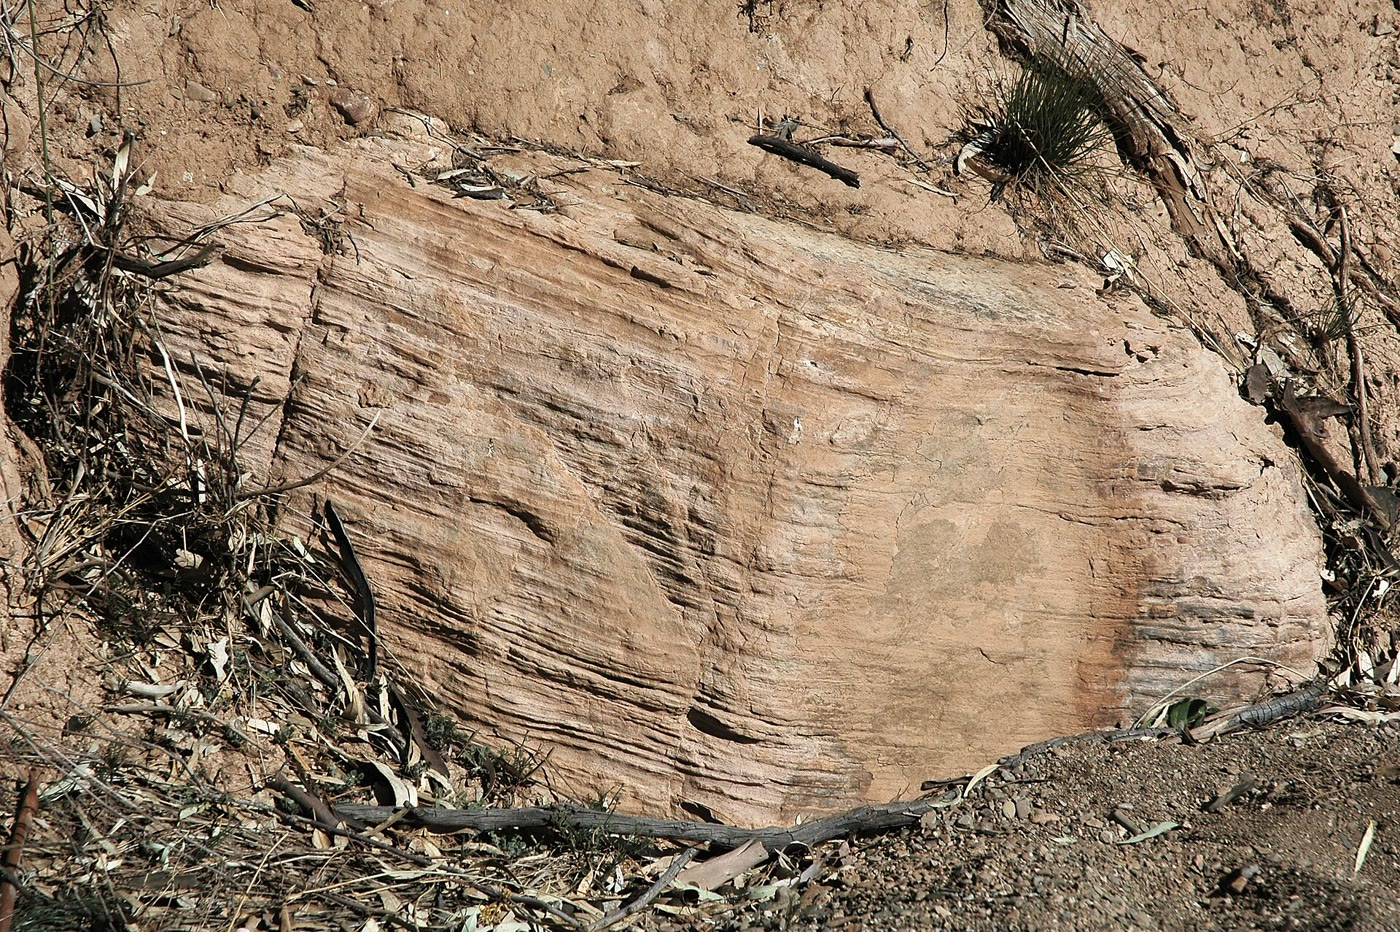
\includegraphics[width=0.66\linewidth]{images/book4/b2-18-cap-carbonate.jpg}
\par\smallskip{\small كربونات غطائية: دولوستون مصفّح من تكوين نوكالينا،
سلسلة فلندرز، جنوب أستراليا، يرتكز على رواسب تجلّد مارينوي
(الطبقات مائلة). الصورة: \mbox{\textdir TLT James St.~John, CC~BY~2.0 (Wikimedia Commons)}.}
\end{omfigure}

أُرِّخت اليوم كرتان ثلجيتان من الكريوجيني بأعمار اليورانيوم--الرصاص على زركون من الرماد
البركاني وبأعمار الرينيوم--الأوزميوم على طين صفحي غنيّ بالمادة العضوية. فقد بدأ الستيرتي بين 717.5
و\qty{716.3}{Ma} وانتهى بين 659.3 و\qty{658.5}{Ma}: أي \qty{58}{Myr} من الجليد، مع
بداية ونهاية متزامنتين في أنحاء العالم. وبدأ المارينوي بين 649.9
و\qty{639.0}{Ma}، بتأريخ تقريبي، وانتهى بين 636.0 و\qty{634.7}{Ma}: أي
\qty{3}{Myr} على الأقلّ. وتنتهي كلّ منهما بطبقة كربونات غطائية واحدة، لا بعدّة طبقات قط. وتكوينات الحديد،
الغائبة منذ مليار سنة، تعود في الرواسب الجليدية للستيرتي. وقد جاءت كرة ثلجية أسبق
واحدة على الأقلّ، في السيدري نحو \qty{2.4}{Ga}، في زمن \omterm{def:b2:precambrian-earth:goe}{حدث الأكسدة العظيم}؛ وبين
النوبتين، طوال نحو \qty{1.5}{Gyr}، لا تكاد تُعرف صفائح جليدية.
% ledger: hoffman17:ages, hoffman17:cryochrons, hoffman17:cap, hoffman17:models, hoffman17:earlier

\begin{history}[من فرضية غريبة إلى نظرية مؤرَّخة]
في عام 1964 لفت و.~ب.~هارلاند الانتباه إلى أدلّة تجلّد في أواخر ما قبل الكمبري. وفي
عامَي 1968 و1969 وجد م.~إ.~بوديكو، وكذلك و.~د.~سيلرز بنموذج مشابه، أن
\omterm{def:b2:precambrian-earth:ice-albedo}{التغذية الراجعة للجليد والألبيدو} قد تجعل الجليد ينتشر حتى خطّ الاستواء متى تقدّم بما يكفي؛ فبدت
الأرض المتجمّدة كلّيًا حينئذ حالةً لا عودة منها، ومن ثَمّ حالةً لم تحدث قط.
وفي عام 1981 وصف ج.~ووكر وب.~هايز وج.~كاستينغ المنظّم الحراري لتجوية السيليكات،
ولاحظوا أن ثاني أكسيد الكربون البركاني يتراكم على الأرض المتجمّدة حتى يذوب
الجليد: فالحالة قادرة على إنهاء نفسها. وفي عام 1992 اقترح ج.~ل.~كيرشفنك أنها
حدثت فعلًا، وسمّاها «\omterm{def:b2:precambrian-earth:snowball}{الأرض الكرة الثلجية}»؛ وفي عام 1998 نشر ب.~ف.~هوفمان وزملاؤه
\mbox{\textdir TLT ``A Neoproterozoic Snowball Earth''}، وصارت الحقب الجليدية الشاملة تُسمّى «الكريوكرونات». ولم يكن
أيّ راسب جليدي كريوجيني قد أُرّخ إشعاعيًا قبل عام 2004؛ والتواريخ أعلاه هي
عمل السنين التي تلت.
\end{history}
% ledger: hoffman17:history

البراكين هي المخرج. فعلى أرض يغطّيها الجليد يكاد المطر والأنهار يتوقّفان، ومعهما تجوية
السيليكات، ويتراكم ثاني أكسيد الكربون الذي تطلقه البراكين في الهواء
حتى تذيب دفيئته الجليد.

\begin{proposition}[تراكم ثاني أكسيد الكربون]\label{prop:b2:precambrian-earth:co2}
إذا أُطلق ثاني أكسيد الكربون بمعدّل $F$ (كتلة في السنة) في غلاف جوي كتلته
$M_{\text{a}}$ وكتلته المولية المتوسطة $\bar M$، دون أي مصرف، فإن الزمن اللازم لرفع نسبة خلطه
الحجمية من الصفر تقريبًا إلى $x$ هو
\[
  \tau = \frac{x}{1 - x}\,\frac{M_{\mathrm{CO_2}}}{\bar M}\,\frac{M_{\text{a}}}{F} .
\]
\end{proposition}

\begin{proof}
يحوي الغلاف الجوي $n = M_{\text{a}}/\bar M$ مولًا من الغازات الأخرى. وإضافة $n_c$ مولًا من
ثاني أكسيد الكربون تجعل نسبة خلطه $x = n_c/(n + n_c)$، فيكون $n_c = n\,x/(1 - x)$، وكتلتها
$n_c M_{\mathrm{CO_2}}$؛ وبالمعدّل $F$ يستغرق ذلك $\tau = n_c M_{\mathrm{CO_2}}/F$.
\end{proof}

\begin{example}[كم يستغرق الخروج؟]\label{ex:b2:precambrian-earth:escape}
أعلى تقدير مفضَّل للإطلاق البركاني الحالي هو \qty{0.26}{Gt} من ثاني أكسيد
الكربون في السنة. وتتراوح تقديرات
نسبة الخلط اللازمة لإنهاء كرة ثلجية كريوجينية من 0.01 إلى 0.1. ومع $M_{\text{a}} =
\qty{5.1e18}{kg}$ و$\bar M = \qty{28.97}{g.mol^{-1}}$ و$M_{\mathrm{CO_2}} =
\qty{44.01}{g.mol^{-1}}$، تستغرق $x = 0.01$ مدّة $\frac{0.01}{0.99}\times1.519\times\qty{5.1e18}{kg}
/ \qty{0.26e12}{kg.yr^{-1}} = \qty{0.30}{Myr}$، وتستغرق $x = 0.1$ مدّة \qty{3.3}{Myr}.
\end{example}
% ledger: usgs:volcanic-co2, hoffman17:co2, earth:Matm, earth:Mmol, ciaaw:abridged-2024
% values: co2_t001_Myr 0.301, co2_t01_Myr 3.311 (precambrian.py)

عمود من ثاني أكسيد الكربون الخالص يزن \qty{1}{bar} فوق الأرض كلّها يستغرق
\qty{20}{Myr} بالمعدّل نفسه، وهو الرقم الذي أعطاه ووكر وهايز وكاستينغ. وبضعة ملايين من السنين
زمن طويل، لكن الستيرتي دام \qty{58}{Myr}. فإمّا أن العتبة كانت أعلى، وإمّا أن
انطلاق الغازات كان أقلّ، وإمّا أن الأرض المتجمّدة كانت لا تزال تملك مصارف: وتجوية قاع البحر الفتيّ،
التي لا تتوقّف تحت الجليد، مرشّحة لذلك. وفي نموذج توازن الطاقة يحتاج الخروج إلى
أن تنخفض الانبعاثية الفعّالة للكرة الثلجية حتى تبلغ حرارتها \qty{263}{K}: فتحت
شمس الكريوجيني، \qty{94}{\percent} من شمس اليوم، من 0.616 إلى 0.472، أي احتباس إضافي قدره
نحو \qty{39}{W.m^{-2}} (\cref{exo:b2:precambrian-earth:10}).
% ledger: hoffman17:co2, hoffman17:models, usgs:volcanic-co2
% values: one_bar_Myr 19.98, eps_melt_094 0.4716, forcing_melt_094 39.1 (precambrian.py)

حين ينفتح الجليد أخيرًا عند خطّ الاستواء، تعمل التغذية الراجعة بالعكس: فالبحر الداكن يمتصّ مزيدًا من
ضوء الشمس، ويتراجع الجليد، وتجعل النماذج خطّ الجليد يندفع نحو القطبين في نحو
\qty{2}{kyr}. فتجد الأرض نفسها عندئذٍ بدفيئة هائلة فوق سطح داكن، في مرحلة لاحقة
حارّة. والتجوية، السريعة جدًا في ذلك المناخ، تصبّ الكالسيوم والمغنيسيوم والبيكربونات في
البحر، حيث تترسّب \omterm{def:b2:precambrian-earth:snowball}{الكربونات الغطائية} بينما تغمر مياه الذوبان الأرصفة؛ ويستغرق الأمر
نحو عشرة ملايين سنة لسحب ثاني أكسيد الكربون من جديد. والصفائح الجليدية \omterm{def:b2:precambrian-earth:snowball}{والكربونات
الغطائية}، وتكوينات الحديد والأعمار المتزامنة، هي ما يجعل معظم الجيولوجيين يقبلون اليوم
بأن الكرات الثلجية الكريوجينية حدثت، وإن ظلّ مدى شدّتها --- أي هل بقي حزام من الماء
المفتوح عند خطّ الاستواء، كما تقترح نماذج «الحزام المائي» --- موضع نقاش.
% ledger: hoffman17:hysteresis, hoffman17:cap, hoffman17:debate

\section*{التمارين}\label{sec:b2:precambrian-earth:exercises}

معطيات التمارين، ما لم يُذكر غير ذلك: $\sigma = \qty{5.670e-8}{W.m^{-2}.K^{-4}}$؛
و$S_0 = \qty{1361}{W.m^{-2}}$؛ وألبيدو اليوم 0.294 ومتوسط حرارة السطح \qty{288}{K}؛
وألبيدو الكرة الثلجية 0.6؛ والمنحدر من \qty{263}{K} إلى \qty{283}{K}؛ والانبعاثية الفعّالة اليوم
0.616؛ وقانون غوف $L/L_0 = 1/(1 + 0.4\,t/t_\odot)$ لزمن $t$ قبل الحاضر، مع $t_\odot =
\qty{4.567}{Gyr}$؛ وخطّ سيولة \omterm{def:b2:precambrian-earth:greenstone}{الكوماتيت} \qty{1616}{\celsius} عند \qty{32.2}{\percent} من أكسيد المغنيسيوم،
والميل \qty{18.0}{\celsius} لكل واحد في المئة؛ وأعمار النصف: \ce{^{238}U} \qty{4.468}{Gyr}، و\ce{^{235}U}
\qty{0.704}{Gyr}، و\ce{^{232}Th} \qty{14.0}{Gyr}، و\ce{^{40}K} \qty{1.248}{Gyr}.
% ledger: const:sigma, earth:TSI, earth:albedo, earth:Tsurf, hoffman17:models, gough81:luminosity, connelly12:cai, so16:liquidus, iaea:isotopes

\begin{exercise}[$\star$]\label{exo:b2:precambrian-earth:1}
(أ) كم دام \omterm{def:b2:precambrian-earth:eons}{الدهر الجهنمي}، \omterm{def:b2:precambrian-earth:eons}{والدهر السحيق} \omterm{def:b2:precambrian-earth:eons}{ودهر الحياة الطليعية}؟ (ب) ما الكسر الذي تمثّله الدهور الثلاثة معًا من عمر
الأرض؟ (ج) كم كان عمر الأرض حين تبلور أقدم زركون معروف، وحين
تكوّنت أقدم الصخور؟
\end{exercise}

\begin{exercise}[$\star$]\label{exo:b2:precambrian-earth:2}
تطلق الأرض السيليكاتية الكلّية اليوم، لكل كيلوغرام، \qty{1.917}{pW} من \ce{^{238}U}،
و\qty{0.082}{pW} من \ce{^{235}U}، و\qty{2.089}{pW} من \ce{^{232}Th} و\qty{0.818}{pW} من
\ce{^{40}K} ($\qty{1}{pW} = \qty{e-12}{W}$). (أ) أوجد كلّ إسهام قبل \qty{3}{Gyr}،
والمجموع. (ب) بأيّ عامل انخفض إنتاج الحرارة منذ ذلك الحين؟ (ج) أيّ النظائر يتصدّر
اليوم، وأيّها كان يتصدّر حينئذ؟
\end{exercise}

\begin{exercise}[$\star$]\label{exo:b2:precambrian-earth:3}
استعمل مقياس الحرارة الكوماتيتي. (أ) ما خطّ سيولة كوماتيت فيه
\qty{28}{\percent} من أكسيد المغنيسيوم؟ (ب) ما محتوى أكسيد المغنيسيوم الذي يوافق \qty{1500}{\celsius}؟ (ج) مسيل
ذو نسيج سبينيفكس محتوى الصخر الكلّي فيه من أكسيد المغنيسيوم \qty{38}{\percent}. لماذا لا ينبغي أن يُقرأ خطّ سيولته
من الخطّ؟
\end{exercise}

\begin{exercise}[$\star$]\label{exo:b2:precambrian-earth:4}
رتّب ما يلي وأعطِ أعمارها التقريبية: \omterm{def:b2:precambrian-earth:goe}{حدث الأكسدة العظيم}، وأولى
الستروماتوليتات، ونهاية تجلّد مارينوي، وآخر الكوماتيتات الشائعة، وأقدم
الصخور، والارتفاع الثاني للأكسجين، وأولى أحافير الإدياكاري، ونهاية بنى القباب والعوارض
في بيلبارا.
\end{exercise}

\begin{exercise}[$\star\star$]\label{exo:b2:precambrian-earth:5}
(أ) تحقّق من أن الانبعاثية الفعّالة للأرض اليوم 0.616. (ب) أوجد توازن الكرة الثلجية
تحت شمس اليوم. (ج) بيّن أن التوازن الأوسط، \qty{275.5}{K}، يحقّق
$R = E$ في حدود \qty{0.5}{W.m^{-2}}. (د) أوجد ميلَي $R$ و$E$ هناك، واستنتج
أنه غير مستقرّ.
\end{exercise}

\begin{exercise}[$\star\star$]\label{exo:b2:precambrian-earth:6}
(أ) باستعمال قانون غوف، أوجد ضوء الشمس قبل \qty{2.4}{Ga} وقبل \qty{0.65}{Ga} كسرين
من ضوء اليوم. (ب) في النموذج، هل يمكن مناخ دافئ عند كلّ من التاريخين مع انبعاثية اليوم؟
(ج) يكتب هوفمان وزملاؤه أن شمس السيدري كانت أخفت بنحو \qty{10}{\percent} من
شمس الكريوجيني. تحقّق.
\end{exercise}

\begin{exercise}[$\star\star$]\label{exo:b2:precambrian-earth:7}
دام الستيرتي من \qty{716.9}{Ma} إلى \qty{658.9}{Ma} (منتصفا الفترتين المؤرَّختين)،
والمارينوي من \qty{644.5}{Ma} إلى \qty{635.4}{Ma}. (أ) أوجد مدّتيهما والفترة
بين الجليدية بينهما. (ب) ما الكسر من عصر الكريوجيني، من 720 إلى \qty{635}{Ma}،
الذي غطّى فيه الجليد الأرض، بحسب هذه الأرقام؟ (ج) لماذا لا تكون مدّة المارينوي إلا رقمًا
تقريبيًا؟
\end{exercise}

\begin{exercise}[$\star\star$]\label{exo:b2:precambrian-earth:8}
(أ) كم تستغرق البراكين، بمعدّل \qty{0.26}{Gt} في السنة ودون أي مصرف، لترفع الهواء إلى
نسبة خلط لثاني أكسيد الكربون قدرها 0.05؟ (ب) كم ضعفًا من قيمة عام 1750، \qty{278}{ppm}، يمثّل ذلك؟ (ج) لو امتصّت تجوية قاع
البحر نصف الإطلاق، فكم يستغرق ذلك؟
\end{exercise}
% ledger: usgs:volcanic-co2, earth:Matm, earth:Mmol, ciaaw:abridged-2024, ipcc:erf-2xco2

\begin{exercise}[$\star\star$]\label{exo:b2:precambrian-earth:9}
يحوي دياميكتيت من الطليعي الحديث حجارة مخدّشة، يقع بعضها في طين دقيق التصفّح
ينثني نحو الأسفل تحتها. (أ) ماذا يدلّ عليه الانثناء؟ (ب) خطّ عرضه القديم
\ang{10}. لماذا يهمّ هذا فرضية الكرة الثلجية؟ (ج) يعلوه مباشرةً
دولوستون وردي مصفّح سمكه بضعة أمتار. ما هو، وماذا يسجّل؟
\end{exercise}

\begin{exercise}[$\star\star\star$]\label{exo:b2:precambrian-earth:10}
تحت شمس الكريوجيني، $S = 0.94\,S_0$. (أ) بيّن أن الحالة الدافئة في النموذج لا تزال
موجودة، بالكاد، لكن الكرة الثلجية موجودة أيضًا. (ب) أوجد حرارة الكرة الثلجية مع
انبعاثية اليوم. (ج) أوجد الانبعاثية التي تبلغ عندها الكرة الثلجية \qty{263}{K}
وتذوب. (د) حوّل تغيّر الانبعاثية إلى احتباس إضافي للإشعاع طويل الموجة عند
\qty{263}{K}، بوحدة \unit{W.m^{-2}}.
\end{exercise}

\begin{exercise}[$\star\star\star$]\label{exo:b2:precambrian-earth:11}
(أ) باستعمال نقطتي التحوّل في \cref{prop:b2:precambrian-earth:tipping}، بيّن أن عرض
حلقة التخلّف، $S_{\text{m}}/S_{\text{f}}$، لا يتوقّف على الانبعاثية،
واحسبه. (ب) ما الذي يجعل الحلقة أضيق؟ (ج) لماذا لا تستطيع الكرة الثلجية أن تذوب إلا بعيدًا عن
الأحوال التي تجمّدت فيها؟
\end{exercise}

\begin{exercise}[$\star\star\star$]\label{exo:b2:precambrian-earth:12}
اشتقّ الثابت الزمني لنموذج توازن الطاقة قرب التوازن الدافئ، $\tau =
C/(E'(T^*) - R'(T^*))$، واحسبه لطبقة محيطية مختلطة عمقها \qty{50}{m}، كثافتها
\qty{1025}{kg.m^{-3}} وحرارتها النوعية \qty{3992}{J.kg^{-1}.K^{-1}}. ماذا يحدث للثابت $\tau$ كلّما
اقترب ضوء الشمس من نقطة التحوّل اليسرى، في هذا النموذج وفي نموذج يتغيّر ألبيدوه
تغيّرًا سلسًا مع درجة الحرارة؟
\end{exercise}
% ledger: noaa:seawater-1025, teos10:cp0

\begin{problem}[{مسألة نهاية الأسبوع --- أرض فتيّة أسخن}]\label{pb:b2:precambrian-earth:1}
تتبع هذه المسألة الأرض الفتيّة من باطنها إلى هوائها. استعمل معطيات
التمارين؛ وتحوي الأرض السيليكاتية الكلّية \qty{0.0203}{ppm} من اليورانيوم، و\qty{0.0795}{ppm} من
الثوريوم و\qty{240}{ppm} من البوتاسيوم كتليًا، وتطلق نظائرها \qty{95.13}{\micro W}
(\ce{^{238}U})، و\qty{568.47}{\micro W} (\ce{^{235}U})، و\qty{26.28}{\micro W} (\ce{^{232}Th})
و\qty{28.47}{\micro W} (\ce{^{40}K}) لكل كيلوغرام من النظير. وكتليًا، يتكوّن اليورانيوم من
\qty{99.29}{\percent} \ce{^{238}U} و\qty{0.711}{\percent} \ce{^{235}U}، ويحوي البوتاسيوم
\qty{0.0120}{\percent} \ce{^{40}K}. دوّر إلى ثلاثة أرقام معنوية.

\noindent\textbf{الجزء الأول --- الحرارة من الداخل.}
\begin{enumerate}
  \item أوجد الحرارة التي يطلقها اليوم كلّ نظير لكل كيلوغرام من الأرض السيليكاتية الكلّية، بوحدة
        \unit{pW.kg^{-1}}.
  \item أوجد المجموع.
  \item أوجد ثابت التفكّك لكلّ نظير، بوحدة \unit{Gyr^{-1}}.
  \item أوجد كلّ إسهام قبل \qty{2.7}{Gyr}، حين ثارت كوماتيتات بايك هيل.
  \item أوجد المجموع حينئذ، ونسبته إلى مجموع اليوم.
  \item أيّ النظائر أعطى أكثر الحرارة حينئذ؟ ولماذا يعطي القليل جدًا اليوم؟
\end{enumerate}

\noindent\textbf{الجزء الثاني --- شمس \omterm{def:b2:precambrian-earth:eons}{الدهر السحيق}.}
\begin{enumerate}[resume]
  \item بقانون غوف، أوجد ضوء الشمس قبل \qty{2.7}{Ga} كسرًا من ضوء اليوم،
        وبوحدة \unit{W.m^{-2}}.
  \item أوجد التوازن الدافئ عند ضوء الشمس ذاك مع انبعاثية اليوم. هل هو حالة دافئة صالحة
        في النموذج؟
  \item أوجد توازن الكرة الثلجية عند ضوء الشمس ذاك.
  \item ما الانبعاثية الفعّالة التي تُبقي الأرض عند \qty{288}{K} مع الألبيدو الدافئ؟
  \item كان ثاني أكسيد الكربون وحده قادرًا على ذلك عند 0.004 إلى \qty{0.03}{bar} عند \qty{2.5}{Ga}.
        في غلاف جوي من نحو \qty{1}{bar}، كم ضعفًا من قيمة عام 1750، \qty{278}{ppm}، يمثّل
        ذلك؟
  \item سمِّ العملية التي أبقت ثاني أكسيد الكربون عند هذا المستوى مئات ملايين
        السنين.
\end{enumerate}

\noindent\textbf{الجزء الثالث --- كرة ثلجية ونهايتها.}
\begin{enumerate}[resume]
  \item الكرة الثلجية الأولى، قبل \qty{2.4}{Ga}: أوجد ضوء الشمس حينئذ كسرًا من ضوء اليوم.
        هل لا تزال الحالة الدافئة في النموذج ممكنة مع انبعاثية اليوم؟
  \item بمعدّل \qty{0.26}{Gt} من ثاني أكسيد الكربون في السنة، كم يستغرق بلوغ نسبة خلط
        قدرها 0.1؟
  \item لو كانت العتبة تحت شمس السيدري الأخفت ضعف ذلك، 0.2، فكم يستغرق؟
  \item أيّ صخر يسجّل نهاية الكرة الثلجية، وكيف؟
  \item لماذا تحتاج تكوينات الحديد في الستيرتي إلى محيط بلا أكسجين تحت الجليد؟
\end{enumerate}

\noindent\textbf{الجزء الرابع --- مقياس الحرارة الكوماتيتي.}
\begin{enumerate}[resume]
  \item تحقّق من ميل الخطّ الكوماتيتي من التجربتين.
  \item كان في سائل كوماتيتي من بايك هيل \qty{30}{\percent} من أكسيد المغنيسيوم. أوجد خطّ سيولته.
  \item أوجد خطّ سيولة كوماتيت باربرتون، \qty{32.2}{\percent} من أكسيد المغنيسيوم.
  \item أوجد خطّ سيولة بازلت ظهرة أوّلي فيه \qty{12}{\percent} من أكسيد المغنيسيوم.
  \item لو استُعمل بدلًا من ذلك ميل كيلاويا، \qty{20}{\celsius} لكل واحد في المئة، فكم تكون حرارة
        البازلت، انطلاقًا من نقطة باربرتون؟ وما أثر اختيار الميل؟
  \item لماذا يكون فرق الحرارة بين نوعي الحمم أكبر من فرق درجة
        الحرارة الكامنة بين وشاح \omterm{def:b2:precambrian-earth:eons}{الدهر السحيق} ووشاح اليوم؟
  \item خلاصة: بكم كانت أسخن حمم كوماتيتية في \omterm{def:b2:precambrian-earth:eons}{الدهر السحيق} أسخن من بازلت أوّلي
        لظهرات اليوم؟
\end{enumerate}
\end{problem}
% ledger: ms95:pm-trace, dye:isotope-heat, iaea:isotopes, gough81:luminosity, cz20:archean-air, ipcc:erf-2xco2, usgs:volcanic-co2, hoffman17:co2, so16:liquidus, helz98:glass-thermometer, pierru22:komatiite
